\documentclass[12pt]{article}
\usepackage[utf8]{inputenc}
\usepackage[T2A]{fontenc}
%\usepackage{libertine}
%\usepackage{pscyr}
\usepackage[a4paper, left = 2.5cm,right = 2.5cm,top = 2.5cm,bottom = 3cm]{geometry}
\usepackage[english,russian]{babel}
\usepackage{amsmath}
\usepackage{amssymb}
\usepackage{amsfonts}
\usepackage[final]{graphicx}
\usepackage[linktocpage=true, colorlinks=true, linkcolor = blue, citecolor = red]{hyperref}
\usepackage{cmap}
\usepackage{xfrac}
%\usepackage[titletoc]{appendix}
\usepackage{pgfplots}
\usepackage{cite}
\newcommand{\eprint}{}

%\linespread{1.2}

\newcommand{\bq}{\begin{equation}}
\newcommand{\eq}{\end{equation}}

\usepackage{tikz}

%%%%%%%%%%
\newcommand{\dd}{\partial}
\newcommand{\de}{\delta}
\newcommand{\m}{\mu}
\newcommand{\n}{\nu}
\newcommand{\ls}{\left(}
\newcommand{\rs}{\right)}
\newcommand{\la}{\lambda}
\newcommand{\ka}{\varkappa}
\newcommand{\ga}{\gamma}
\newcommand{\si}{\sigma}
\newcommand{\ta}{\tau}
\newcommand{\al}{\alpha}
\newcommand{\be}{\beta}
\newcommand{\ff}{\varphi}
\newcommand{\te}{\theta}

\newcommand{\disn}[2]{$$\displaylines{\refstepcounter{equation}%
            \label{#1}\hskip 1em minus 1em #2\hfilneg}$$}
\newcommand{\nom}{\hfil\hskip 1em minus 1em (\theequation)}
\newcommand{\no}{\hfil \hskip 1em minus 1em\phantom{(\theequation)}%
            \hfilneg\cr\hfilneg\hskip 1em minus 1em\hfil}
\newcommand{\ns}{\hfill\cr\hfill}

%%%%%%%%%%


\begin{document}

\title{Explisit isometric embeddings of collapsing black hole}
\author{
A.~D.~Kapustin\thanks{E-mail: sashakapusta96@gmail.com},
S.~A.~Paston\thanks{E-mail: pastonsergey@gmail.com}\\
{\it Saint Petersburg State University, Saint Petersburg, Russia}
}
\date{\vskip 15mm}
\maketitle

\begin{abstract}
В этой работе ищутся явные вложения наименьшей размерности для метрики коллапсирующего сферически симметричного облака пылевидной материи, образующего Шварцшильдовскую черную дыру. В работе рассматриваются два подхода, в одном из которых находится глобальное семимерное вложение с изломом, а в другом локальное семимерное, также содержащее излом. Однако для частного случая во втором подходе удается найти гладкое шестимерное вложение, покрывающее все области многообразия.
\end{abstract}

\clearpage

\section{Введение}
Как известно (см., например, \cite{goenner}), любое (псевдо)риманово многообразие размерности $d$ может быть \emph{изометрически} вложено в \emph{плоское} объемлющее пространство размерности $N \geqslant d(d+1)/2$ как минимум локально.
В результате многообразие можно описывать функцией вложения $y^a(x^\mu)$, а метрику считать \emph{индуцированной}
\bq\label{s1}
	g_{\mu \nu} = (\partial_{\mu} y^a) (\partial_{\nu} y^b) \eta_{ab},
\eq
где $\eta_{ab}$ -- плоская метрика объемлющего пространства; здесь и далее $\mu,\nu=0,...,d-1$; $a,b=1,...,N$.
Такой способ описания многообразия может оказаться наглядным и полезным для изучения его структуры, однако он требует отыскания явного вида функции вложения для заданной метрики $g_{\mu\nu}$, т.е. решения дифференциального уравнения \eqref{s1} относительно $y^a$. Изучение структуры многообразия особенно актуально в отношении черных дыр, так как соответствующие им многообразия обычно имеют нетривиальную структуру.

Для невращающейся незаряженной черной дыры, соответствующей метрике Шварцшильда, первое явное вложение было построено еще в 1921 году \cite{kasner3},
однако оно (равно как и вложение \cite{fudjitani}) применимо только вне горизонта, поэтому для изучения структуры многообразия непригодно.
Наиболее полезное для такой цели вложение было предложено в 1959 году в работе \cite{frons}, оно, оставаясь везде гладким, применимо
как вне, так и внутри горизонта, причем соответствует максимальному аналитическому расширению решения Шварцшильда,
которое включает в себя две области вне горизонта (две вселенные) и две области под горизонтом, соответствующие черной и белой дырам.
Кроме перечисленных, известно еще три так называемых "минимальных"{} (т.е. соответствующих минимально возможной размерности
объемлющего пространства, в данном случае равной 6 \cite{kasner2}) вложения \cite{davidson,statja27} метрики Шварцшильда, которые покрывают
половину упомянутого максимального аналитического расширения -- например, совокупность области вне горизонта и области под горизонтом, соответствующей черной дыре,
см. подробности в \cite{statja27}.
Отметим, что только именно эти две области имеют место, если вместо максимального аналитического расширения, соответствующего \emph{вечной}
черной дыре, рассматривать риманово пространство, соответствующее черной дыре, возникающей в результате коллапса.

Задача поиска минимальных \emph{глобальных} (т.е. гладких при всех значениях радиуса, включая точки горизонтов)
вложений для невращающейся заряженной черной дыры Райсснера-Нордстрема рассматривалась в работе \cite{statja30}.
Было построено три варианта вложения, которые могут использоваться как для случая nonextremal charged black hole,
так и для случаев extremal and hyperextremal one. Обобщение на случай присутствия космологической постоянной изучалось в  работе \cite{statja40}.
Для физически более интересного случая вращающейся черной дыры Керра, равно как и для его обобщения -- заряженной вращающейся черной дыры Керра-Ньюмена,
задача построения явных вложений оказывается гораздо более сложной из-за более маленькой группы симметрии задачи.
Известны только записанные в неявном виде (в виде двух дифференциальных уравнений на две неизвестные компоненты функции вложения)
локальные вложения в 9-мерное объемлющее пространство \cite{kuzeev} и \cite{kuzeevRN} (для метрик Керра и Керра-Ньюмена соответственно)
и 14-мерное вложение метрики Керра, предложенное в работе \cite{gr-qc/0503079}.

Нахождение явных вложений для физически интересных решений теории гравитации может быть полезным
еще и с точки зрения изучения описания гравитации в рамках теории вложения -- гравитации Редже-Тейтельбойма, впервые предложенной в работе \cite{regge}.
В рамках этого подхода именно функция вложения $y^a(x)$ является независимой переменной вместо метрики,
которая выражается формулой \eqref{s1}.
После \cite{regge} возможность использования идеи изометрического вложения для описания гравитации, в том числе и в связи с ее квантованием,
неоднократно обсуждались в работах разных авторов, см., например,
работы \cite{deser,pavsic85let,tapia,davkar,statja18,rojas09,statja25,faddeev,statja51}.
Явные вложения римановых многообразий с горизонтами также используются при анализе связи между излучением Хокинга
и излучением Унру, соответствующим движению наблюдателя в объемлющем пространстве \cite{deserlev98,deserlev99,statja36}.
Подробный список литературы, связанной с теорией вложения и смежными с ней вопросами, может быть найден в обзоре \cite{tapiaob}.

Сложность задачи построения явных вложений для произвольного четырехмерного пространства-времени связана с тем, что
необходимо решать систему $10$ дифференциальных уравнений  в частных производных \eqref{s1} относительно функции вложения $y^a(x^\mu)$,
зависящей от $4$ координат $x^\mu$.
Задача упрощается, если у многообразия присутствуют дополнительные симметрии.
Их наличие позволяет использовать конструктивный метод построения явных вложений \cite{statja27}, который при
достаточно большой симметрии может свести задачу к решению системы ОДУ.
Именно так происходит для метрик Шварцшильда и Райсснера-Нордстрема, обладающих симметрий $SO(3)\times T^1$, где $T^1$ здесь обозначает трансляционную симметрию
относительно сдвигов времени. Аналогична ситуация (см.~\cite{statja29}) и для космологических решений --
для метрик всех трех моделей FRW, обладающих симметриями: $SO(4)$ для закрытой модели, $SO(1,3)$ для открытой модели
и группой движений трехмерной плоскости для пространственно-плоской модели.

Самым, наверное,  интересным с физической точки зрения вариантом черной дыры является черная дыра, возникающая в результате коллапса,
при котором облако материи сжимается, образуя черную дыру динамически. В таком процессе происходит образование горизонта
и поэтому особенно интересным становится изучение структуры соответствующего многообразия, а значит актуальной становится
задача постоения явного вложения для этого случая.
Даже если пренебречь вращением, т.е. считать, что вне области нахождения материи метрика определяется
решением Шварцшильда, то построить явное вложение для соответствующей этому случаю метрики оказывается
сложной задачей. Именно построению таких вложений посвящена настоящая работа, до сих пор они не были известны.
Для упрощения задачи мы берем простейший вариант поведения коллапсирующей материи, рассматривая коллапс
состоящего из пылевидной материи однородного шара.

Группой симметрии этой задачи является $SO(3)$ и эта симметрия оказывается недостаточно богатой для сведения задачи
к решению системы ОДУ в рамках метода \cite{statja27}. Однако, если рассматривать многообразие как совокупность двух частей --
содержащей материю (сжимающийся или расширяющийся пылевидный шар) и не содержащей ее (область вне этого шара), то для каждой
из частей симметрия оказывается выше и это может упростить задачу. Для области вне шара метрика согласно известной теореме Биркгофа
представляет собой метрику Шварцшильда, а значит обладает симметрией $SO(3)\times T^1$ и мы для нее знаем
упомянутый выше ряд вложений. Для области же внутри шара, метрика соответствует одной из моделей FRW, см., например, \cite{landavshic2},
а значит, тоже обладает расширенной симметрией соответствующего типа и вложения такой метрики также известны \cite{robertson1933}.

Такая ситуация позволяет искать вложения для всего многообразия путем сшивки модифицированных подходящим образом
известных вложений его частей, такой способ применяется в разделе~4. Для более интересного случая динамического
формирования горизонта удается построить вложение в 7-мерное объемлющее пространство с сигнатурой $(+------)$,
однако оно содержит излом (разрыв первой производной функции вложения) и не может быть продолжено
в область сколь угодно больших значений радиуса. Для случая же наличия статического горизонта, когда материя
полностью находится под ним, выходя из белой дыры и падая в черную, построено гладкое вложение
в 6-мерное объемлющее пространство с сигнатурой $(+-----)$.

Альтернативным путем постоения вложения является попытка его построения
единым образом, без использования сшивки известных вложений. Интересно отметить, что и в этом случае
однородность пылевого шара упрощает решение задачи и позволяет найти явный вид вложения для случая коллапса,
т.е. при динамическом формировании горизонта. Такой способ рассуждения применяется в разделе~3.
На этом пути удается построить вложение в 7-мерное объемлющее пространство с сигнатурой $(+-+----)$,
причем оно оказывается гладким.
%В разделе~2 описывается вид метрики, для которой мы будем искать явные вложения,
%и рассматриваются две системы координат, используемых при этом.




\section{Вид метрики и используемые координатные системы}
Запишем выражение для метрики, соответствующее сжимающемуся (или расширяющемуся) пылевидному шару конечного размера.
Эта метрика должна являться решением уравнений Эйнштейна
\begin{equation}
\label{G=T}
	G_{\mu \nu} = \varkappa\, T_{\mu \nu}
\end{equation}
с ТЭИ, соответствующим выбраному типу материи и ее распределению.
Для пылевидной материи ТЭИ выглядит наиболее просто, если использовать систему синхронных сопутствующих координат.
В силу сферической симметрии удобно в качестве двух пространственных координат выбрать углы $\theta$ и $\varphi$.
Оставшуюся времениподобную координату обозначим $\tau$, а пространственноподобную -- $\chi$.

Описанное решение уравнений Эйнштейна можно найти в виде диагональной метрики. Для произвольного распределения материи по радиусу
соответствующий этой метрике квадрат интервала (далее аналогичные формулы будем для краткости называть метрикой) имеет вид \cite{landavshic2}
\bq
\label{metric}
	d s^2 = d \tau^2 - \frac{(r'(\tau, \chi))^2}{1+f(\chi)} d\chi^2 - r^2(\tau, \chi) d \Omega,
\eq
где $d\Omega=d\theta^2+sin^2\theta d\varphi^2$, а
функция $r(\tau, \chi)$ определяется одним из трех способов
\bq
\label{v123}
	r(\tau, \chi) = \left\{
	\begin{matrix}
	\frac{F(\chi)}{2 f(\chi)} H \left( \frac{2(f(\chi))^{\sfrac{3}{2}} }{F(\chi)}(\tau_0(\chi)-\tau)  \right) , \ \ \ \ f(\chi) > 0,\\
	\left( \frac{9F(\chi)}{4} \right)^{\sfrac{1}{3}} \left[ \tau_0(\chi)- \tau \right]^{\sfrac{2}{3}}, \ \ \ \ f(\chi) = 0, \\
	- \frac{F(\chi)}{2 f(\chi)} E \left( \frac{2(-f(\chi))^{\sfrac{3}{2}} }{F(\chi)}(\tau_0(\chi)-\tau) \right), \ \ \ \ f(\chi) < 0.
	\end{matrix} \right.
\eq
Функции $H(x)$ и $E(x)$ служат для обращения параметрических зависимостей
\bq\label{sp4}
H = \ch{\eta}-1,\quad x = \sh{\eta} - \eta;\qquad
E = 1 - \cos{\eta},\quad x = \eta - \sin{\eta},
%	\begin{array}{c}
%	E = 1 - \cos{\eta}, \\
%	x = \eta - \sin{\eta},
%	\end{array} \ \ \ \ \ \ \ \
%	\begin{array}{c}
%	H = \ch{\eta}-1, \\
%	x = \sh{\eta} - \eta,
%	\end{array}
\eq
а функции $F(\chi), f(\chi)$ и $\tau_0(\chi)$ задают распределение плотности материи и ее начальной скорости.
При этом функция $F(\chi)$ имеет смысл радиуса Шварцшильда всей материи, имеющей значение координаты меньшее, чем $\chi$,
а функция $\tau_0(\chi)$ определяет момент времени $\tau$, в который частица с координатой $\chi$
достигнет точки $r=0$, т.е. упадет на образующуюся в результате коллапса сингулярность.

Если потребовать однородности распределения материи в начальный момент, то пространство внутри коллапсирующего шара будет описываться геометрией открытой, пространственно-плоской или закрытой модели Фридмана соответственно выбору первого, второго или третьего способа определения $r(\tau, \chi)$ в формуле (\ref{v123}).
При этом легко заметить, что однородность в каждый момент времени требует одновременности падения всех частиц
в точку $r=0$, вследствие чего функция $\tau_0(\chi)$ должна превращаться в константу и ее можно взять равной нулю выбором времени $\tau$.

Внешнее к шару пространство, согласно теореме Биркгофа, во всех случаях описывается геометрией Шварцшильда.
Поскольку в этой области плотность материи обращается в ноль, значит полная масса материи, имеющей значение координаты меньшее, чем заданное $\chi$,
перестает зависеть от $\chi$. Следовательно, постоянен и радиус Шварцшильда этой материи, а значит подстановка $F(\chi)=const$ в формулу (\ref{metric})
соотвествует переходу к метрике Шварцшильда.

Если плотность материи внутри шара постоянна, а значит, на его границе испытывает скачок,
то метрика (\ref{metric}) будет иметь координатную особенность в виде скачка на границе шара, которую можно устранить
переходом к координатам $(\tau, r, \theta, \varphi)$.
Если совершить такую замену координат, то метрика (\ref{metric}) примет вид
\bq\label{sp1}
	d s^2 = \left( 1- \frac{\dot{r}(\tau, \chi)^2}{1+f(\chi)}\right) d \tau^2 + 2\frac{\dot{r}(\tau, \chi)}{1+f(\chi)}dr d\tau - \frac{dr^2}{1+f(\chi)} - r^2 d\Omega,
\eq
где $\dot{r}(\tau, \chi) \equiv \frac{\partial r(\tau, \chi)}{\partial \tau}$, а $r(\tau, \chi)$ дается \eqref{v123}.
Входящая в \eqref{sp1} через $\dot{r}(\tau, \chi)$ и $f(\chi)$ величина $\chi$
должна быть выражена через независимые координаты $\tau$ и $r$ в соответствии с \eqref{v123}.

Если теперь в \eqref{v123} выбрать вариант $f(\chi)=0$, то ситуация заметно упростится, поскольку
 $r(\tau, \chi)$ и $\dot{r}(\tau, \chi)$ можно будет записать в явном виде. После несложных преобразований метрика примет вид
\bq
\label{metric2}
	d s^2 = \left(1-\frac{F(\tau, r)}{r} \right)d\tau^2 - 2 \sqrt{\frac{F(\tau, r)}{r}}dr d\tau  - dr^2 - r^2 d\Omega,
\eq
где здесь и далее $F(\tau, r)\equiv F(\chi(\tau, r))$.
Пока плотность материи остается конечной, эта метрика, записанная в координатах $(\tau, r, \theta, \varphi)$, будет непрерывной
в силу непрерывности в этом случае функции $F(\chi)$.

Внутри однородного пылевого шара можно считать, что $\tau_0(\chi)=0$ (см. выше, после формулы \eqref{sp4}), что позволяет легко
найти в этой области вид функции $F(\tau, r)$ из \eqref{v123}, случай $f(\chi)=0$. Учитывая, что вне шара $F(\chi)=const$ и предполагая
непрерывность $F(\chi)$, в целом можно записать
\bq\label{sp2}
	F(\tau, r) = \min{ \left( \frac{4r^3}{9\tau^2}, F_0 \right) },
\eq
где $F(\tau, r)=F_0$ вне шара. При этом считаем, что время $\tau$ везде отрицательно и меняется до своего нулевого значения,
которое соответствует завершению коллапса, когда вся материя одновременно достигла точки $r=0$ и образовала сингулярность.

Запись метрики \eqref{metric2} в координатах $(\tau, r, \theta, \varphi)$ будет использоваться при поиске явного вложения в разделе~3.
Возможностью записать метрику в виде \eqref{metric} в синхронной и сопутствующей системе координат мы воспользуемся в разделе~4.



\section{Построение вложения без использования сшивки}
Первый вариант явного вложения будем строить для метрики, взятой в виде (\ref{metric2}),
причем без использования возможности сшивки отдельных вложений для внутренности и внешности шара.
При этом, тем не менее, будем считать, что пылевой шар в каждый момент времени является однородным и можно использовать формулу
\eqref{sp2}, поскольку в этом случае задача упрощается.
Напомним, что даваемая этой формулой величина $F(\tau, r)$ с точностью до множителя дает массу пыли,
содержащейся внутри радиуса $r$ в момент времени $\tau$.
Легко заметить, что с учетом \eqref{sp2} метрика (\ref{metric2}) оказывается непрерывной, однако испытывает излом (разрыв первой производной) на границе шара.

\begin{figure}[h!]
	\centering
	\begin{tikzpicture}[scale=0.7]
		\draw[->] (-5, 0) -- (5, 0)node[below]{$u$};
		\draw[->] (0, -5) -- (0, 5)node[left]{$v$};
		%%
		\draw[->] (4.5, 0.5) -- (5.5, 0.5)node[midway,above]{$r \to \infty$};
		%%
		\begin{scope}
		\clip (7.5, 6) -- (5, 6) -- (0.6, 2.8) .. controls (1, 1) and (1, 0) .. (5, -3) -- (5, -6) -- (7.5, -6) -- cycle;
		\draw[thick, dashed] (-5, -5) -- (5, 5)node[above right]{$r = R$};
		\draw[thick, dashed] (-5, 5) -- (5, -5);
		%%
		\draw (5, 4.9) .. controls (0, 0) and (0, -0) .. (5, -4.9);
		\draw (5, 4.7) .. controls (1.5, 1) and (1.5, -1) .. (5, -4.7);
		\draw (5, 4.5) .. controls (3, 1.5) and (3, -1.5) .. (5, -4.5)node[pos=0.1,below right]{$r=const$};
		%%
		\draw (-5, 4.9) .. controls (0, 0) and (0, -0) .. (-5, -4.9);
		\draw (-5, 4.7) .. controls (-1.5, 1) and (-1.5, -1) .. (-5, -4.7);
		\draw (-5, 4.5) .. controls (-3, 1.5) and (-3, -1.5) .. (-5, -4.5);
		%%
		\draw (4.9, 5) .. controls (0, 0) and (0, 0) .. (-4.9, 5);
		\draw (4.8, 5) .. controls (1, 1) and (-1, 1) .. (-4.8, 5);
		\draw[ultra thick] (4.7, 5) .. controls (2, 2) and (-2, 2) .. (-4.7, 5);
		%%
		\draw (4.9, -5) .. controls (0, 0) and (0, 0) .. (-4.9, -5);
		\draw (4.8, -5) .. controls (1, -1) and (-1, -1) .. (-4.8, -5);
		\draw[ultra thick] (4.7, -5) .. controls (2, -2) and (-2, -2) .. (-4.7, -5);
		\draw (0, -3)node[below right]{$r = 0$};
		%%
		\end{scope}
		\draw (0, 3)node[above right]{$r = 0$};
		\draw[blue, very thick] (5, -3) .. controls (1, 0) and (1, 1) .. (0.6, 2.8);
	\end{tikzpicture}
	\caption{\label{infkrusk}The Kruskal diagram for matter collapsing from infinity.}
\end{figure}
Описываемая метрикой Шварцшильда область вне шара изображена на Рис.~\ref{infkrusk} на диаграмме Крускала.
%Можно представить область пространства, соответствующую константе $F_0$, на диаграмме Крускала, представленной на Рис. \ref{infkrusk}.
Она ограничена мировой линией точки, соответствующей границе шара.
Оставшаяся же часть многообразия, соответствующая внутренности шара, описывается метрикой Фридмана
и на рисунке не показана. Поскольку при переходе от (\ref{metric}) к (\ref{metric2}) было положено $f(\chi)=0$,
то это метрика пространственно-плоской модели Фридмана (см. \eqref{v123} и текст после нее).

Как можно заметить из \eqref{sp2}, граница шара описывается уравнением
\disn{sp3}{
r^3=\frac{9}{4}F_0\tau^2,
\nom}
из которого можно заключить, что $r\to\infty$ при $\ta\to-\infty$,
т.е. размер пылевого шара в прошлом был неограниченно большим.
Это означает, что конструируемое в данном разделе вложение соответствует
коллапсу частиц, прилетающих с пространственной бесконечности.
Отметим, что эта ситуация качественно отличается от рассматриваемой в разделе~4.


%\subsection{Построение вложения для полученной метрики}

Будем искать функцию вложения $y^a(x^\mu)$ в виде совокупности компонент $\{\tilde y^A(\tau,r),\hat y^i(r,\te,\ff)\}$,
где три компоненты $\hat y^i(r,\te,\ff)$ имеют стандартный для сферически-симметричных вложений вид
\begin{align}\label{sp7}
\hat y^1 &= r \cos{\theta}, \nonumber\\
\hat y^2 &= r \sin{\theta} \cos{\varphi},  \\
\hat y^3 &= r \sin{\theta} \sin{\varphi}.\nonumber
\end{align}
Тогда, с учетом структуры формулы индуцированной метрики \eqref{s1},
задача построения явного вложения метрики (\ref{metric2}) сводится к поиску функции вложения двумерной поверхности
$\tilde y^A(\tau,r)$ для метрики
\disn{sp8}{
d s^2 = \left(1-\frac{F(\tau, r)}{r} \right)d\tau^2 - 2 \sqrt{\frac{F(\tau, r)}{r}}dr d\tau.
\nom}
Чтобы упростить этот поиск, введем
вместо переменных $\tau$ и $r$ новые переменные $t = \tau^{\sfrac{2}{3}}$ и $p = r^3/\tau^2$,
так что \eqref{sp2} примет вид
\bq\label{sp6}
F(\tau, r) = \min{ \left( \frac{4}{9}p, F_0 \right) }\equiv\bar F(p).
\eq
Тогда для метрики (\ref{sp8}) получаем выражение
\bq\label{eq10}
	d s^2 = \left(\frac{9}{4} t +f(p) \right) dt^2 + t\, p^{-\sfrac{5}{6}}\sqrt{\bar F(p)} \, dp\, dt,
\eq
где
\bq\label{eq10.1}
f(p) = 3 p^{\sfrac{1}{6}} \sqrt{\bar F(p)}-\frac{9}{4}p^{-\sfrac{1}{3}} \bar F(p).
%=-\frac{9}{4}p^{-\sfrac{1}{3}} \sqrt{\bar F(p)}\ls \sqrt{\bar F(p)}-\frac{4}{3}\sqrt{p}\rs
%,\qquad
%h(p) = \frac{1}{2}p^{-\sfrac{5}{6}}\sqrt{\bar F(p)}.
\eq

Компоненты метрики (\ref{eq10}) являются полиномами по переменной $t$. Это позволяет искать соответствующие ей
компоненты функции вложения $\tilde y^A(t,p)$ также в виде полиномов по $t$, в форме, близкой к использованной при построении
"кубического"{} вложения метрики Шварцшильда в работе \cite{statja27}. Вложение удается найти
для четырехмерного объемлющего пространства с сигнатурой $(+-+-)$. С использованием светоподобных координат
объемлющего пространства $\tilde y^\pm=\tilde y^0\pm\tilde y^1$, его можно записать в виде
\begin{align}\label{sp9}
	\tilde y^{+} &= 2t^3 + \frac{9}{8}t^2+tf(p), \nonumber\\
	\tilde y^2 &=  w(p), \\
	\tilde y^{-} &= t, \nonumber\\
	\tilde y^{3} &= \sqrt{\frac{3}{2}}t^2 -w(p)\nonumber,
\end{align}
где
\disn{sp9.1}{
w(p)=\frac{1}{2\sqrt{6}}\ls\int\!\sqrt{\bar F(p)}\,p^{-\sfrac{5}{6}} dp- f(p)\rs=\ns=
\frac{1}{\sqrt{6}}\te\ls p-\frac{9}{4}F_0\rs
\ls\ls\frac{9}{4}F_0\rs^{\sfrac{1}{2}}p^{\sfrac{1}{6}}+\frac{9}{8}F_0p^{-\sfrac{1}{6}}-\frac{3}{2}\ls\frac{9}{4}F_0\rs^{\sfrac{2}{3}}\rs
\nom}
и $\te(z)$ -- тэта-функция Хевисайда (при вычислении \eqref{sp9.1} использован явный вид \eqref{sp6} функции $\bar F(p)$).

Возвращаясь к более естественным координатам $\tau$, $r$ и объединяя компоненты \eqref{sp9}
с оставшимися компонентами \eqref{sp7} полной функции вложения $y^a(x^\mu)$,
окончательно получаем функцию вложения для метрики (\ref{metric2}) в виде
\begin{align}\label{sp10}
	y^0 &= \tau^2 + \frac{9}{16}\tau^{\sfrac{4}{3}}+\frac{1}{2}\tau^{\sfrac{2}{3}} \ls f\ls\frac{r^3}{\tau^2}\rs+1\rs, \nonumber\\
	y^1 &= \tau^2 + \frac{9}{16}\tau^{\sfrac{4}{3}}+\frac{1}{2}\tau^{\sfrac{2}{3}} \ls f\ls\frac{r^3}{\tau^2}\rs-1\rs, \nonumber\\
	y^2 &=  w\ls\frac{r^3}{\tau^2}\rs, \\
	y^3 &= \sqrt{\frac{3}{2}}\tau^{\sfrac{4}{3}}-w\ls\frac{r^3}{\tau^2}\rs, \nonumber\\
	y^4 &= r \cos{\theta}, \nonumber\\
	y^5 &= r \sin{\theta} \cos{\varphi},  \nonumber\\
	y^6 &= r \sin{\theta} \sin{\varphi},\nonumber
\end{align}
причем объемлющее пространство 7-мерно и обладает сигнатурой $(+-+----)$.
Напомним, что время $\tau$ предполагается всегда отрицательным, а его нулевое значение
соответствует падению всех частиц пылевого шара в точку $r=0$.

Построенное вложение является глобальным в том смысле, что оно остается гладким при всех значениях $r$
и всех $\tau<0$, т.е. до момента образования сингулярности.
Исследуем степень имеющейся гладкости при $\tau<0$.
Прежде всего, при использовании сферических координат нужно проверить отсутствие нарушения гладкости
в точке $r=0$. Для этого достаточно проверить, что компоненты $y^0$,$y^1$,$y^2$,$y^3$ в этой точке конечны и не имеют в ней
нечетных степеней разложении по $r$. Поскольку при $p<9F_0/4$ оказывается $f(p)=p^{\sfrac{2}{3}}$, $w(p)=0$
(см. \eqref{sp6},\eqref{eq10.1},\eqref{sp9.1}), то это оказывается именно так.
Далее, нужно проверить степень гладкости на границе пылевого шара, что соответствует значению аргумента $p=9F_0/4$
функций $f(p)$, $w(p)$.
Как показывает простой анализ тех же формул, в указанной точке функции $f(p)$ и $w(p)$ непрерывны вместе со своими первыми производными,
но их вторые производные испытывают скачок. Графики этих функций при $F_0=1$ приведены на рис.~\ref{graf-f-w}.
\begin{figure}[h!]
\centering
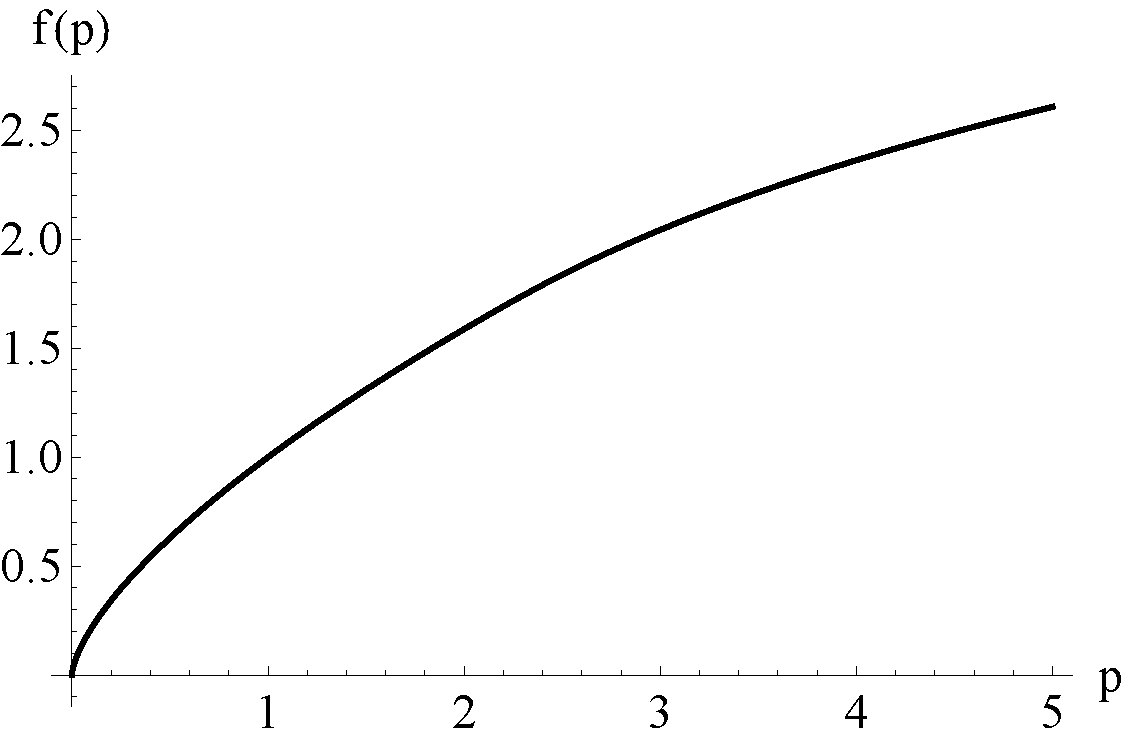
\includegraphics[width=0.45\linewidth]{graf_f.pdf}
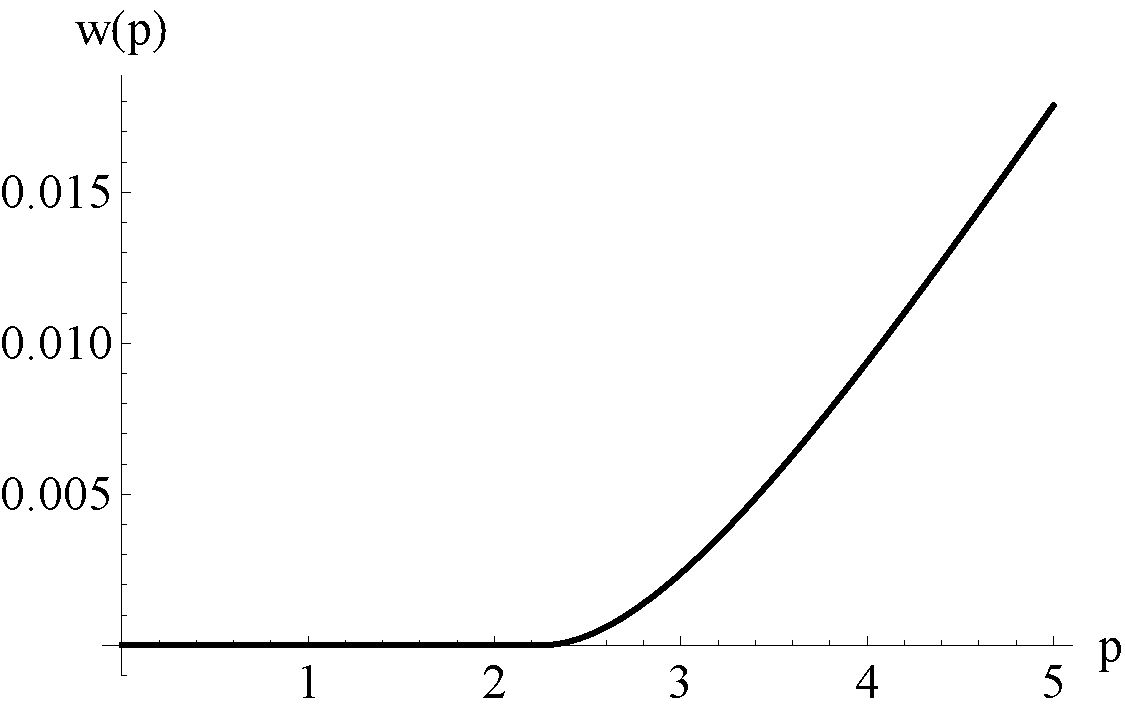
\includegraphics[width=0.45\linewidth]{graf_w.pdf}
\caption{\label{graf-f-w}
Графики функций $f(p)$ и $w(p)$ при $F_0=1$.
}
\end{figure}

Таким образом, построенная явная функция вложения \eqref{sp10} является непрерывно дифференцируемой.
Разрыв ее вторых производных соответствует скачку плотности материи на границе пылевого шара, так что гладкость вложения
соответствует физической постановке задачи. Проекция двумерной поверхности, соответствующей \eqref{sp10}
при фиксированных углах $\theta=\varphi=0$, на трехмерное подпространство $y^0,y^3,y^4$ изображена
на рис.~\ref{pic_emb1}.
\begin{figure}[h!]
\centering
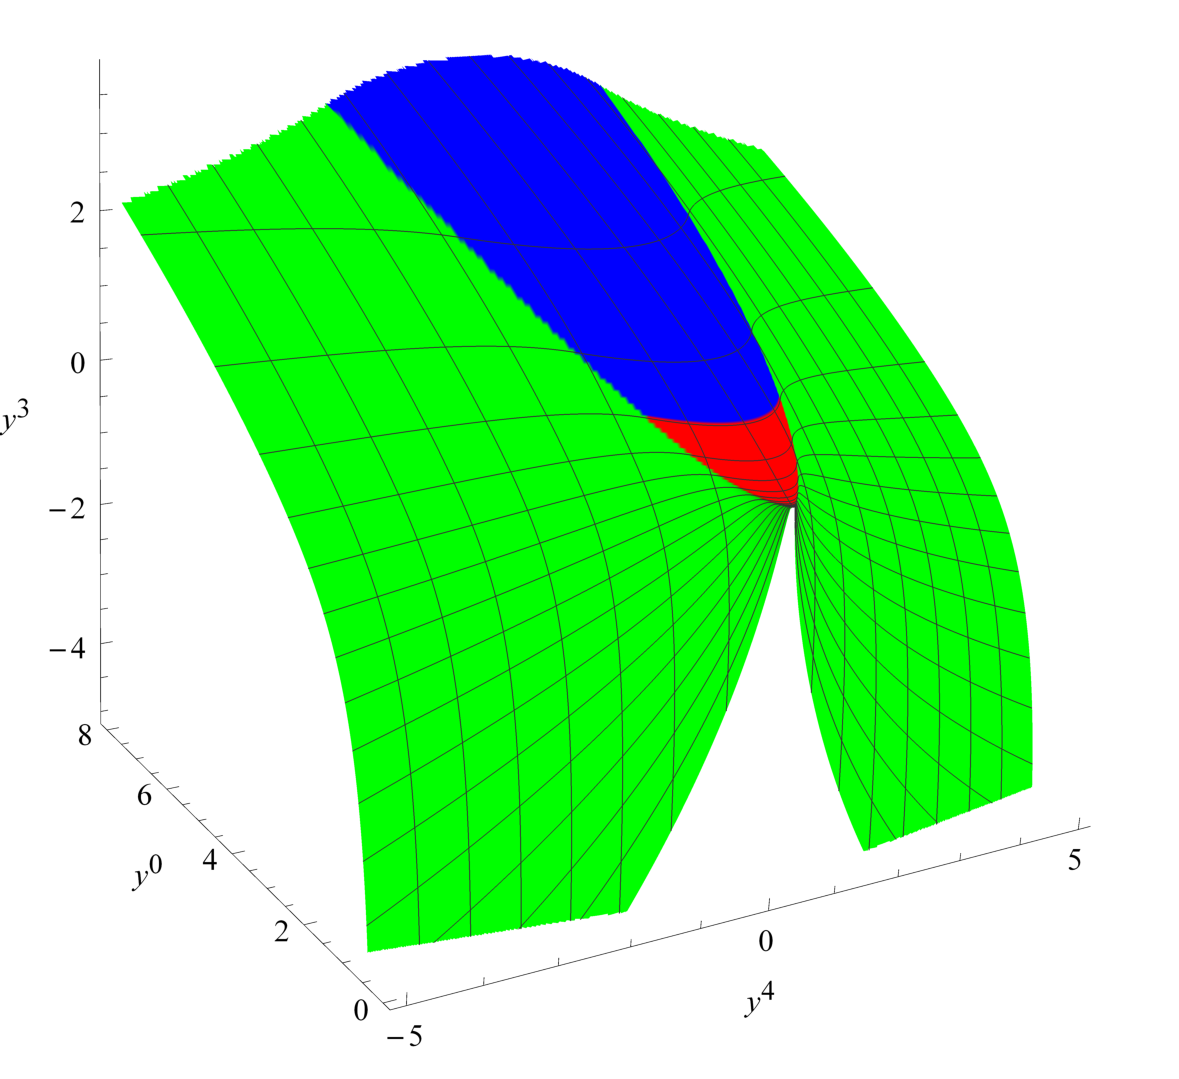
\includegraphics[width=0.55\linewidth]{col_emb-c2.pdf}
\caption{\label{pic_emb1}
Проекция двумерного подмногообразия $\theta=\varphi=0$ вложения \eqref{sp10} на подпространство $y^0,y^3,y^4$.
}
\end{figure}
Зеленым показана область вне пылевого шара, синим и красным -- область пыли до и после образования горизонта, соответственно.
Возникающей в результате коллапса сингулярности соответствует значение $y^0=0$. Интересно отметить, что
в окрестности этой области вид поверхности оказывается сходным с поведением вблизи сингулярности
вложения \cite{robertson1933} для пространственно-плоской модели Фридмана.

Найденный в этом разделе вариант вложения использует объемлющее пространство с двумя времениподобными направлениями,
что можно считать его недостатком с точки зрения попыток придать объемлющему пространству физический смысл.
В следующем разделе мы пытаемся устранить этот недостаток, используя еще один способ построения явного вида вложения,
основанный на сшивке вложений двух частей пространства-времени, соответствующих областям внутри и вне пылевого шара.


\section{Построение вложения с помощью сшивки}
Будем искать вложение для метрики \eqref{metric}, записанной в сопутствующей системе координат, несмотря на то, что
в этих координатах метрика содержит координатную особенность (см. перед формулой \eqref{sp1}).
Мы воспользуемся известными вложениями для областей внутри (метрика Фридмана) и вне  (метрика Шварцшильда)
пылевого шара, модифицировав их таким образом, чтобы полученные функции вложения можно было сшить.

В сопутствующих координатах уравнение движения материи имеет вид $\chi = const$, поэтому можно сказать, что область $0 \leqslant \chi < \chi_0$ содержит материю, область $\chi > \chi_0$ соответствует пустому пространству, а $\chi = \chi_0$ --- граница пылевидного шара.
Выберем $r(\tau, \chi)$ в формуле (\ref{v123}) согласно третьему способу, что соответствует закрытой модели Фридмана в случае однородной плотности материи.
Тогда при выборе функций 
\bq
F(\chi) = \frac{R \sin^3{\chi}}{\sin^3{\chi_0}}, \qquad f(\chi) = -\sin^2{\chi}, \qquad \tau_0(\chi) = const,
\eq
отвечающем постоянной плотности пыли, при $0 \leqslant \chi < \chi_0$, выражение для $r(\tau, \chi)$ примет вид
\bq
	r(\tau, \chi) = \frac{R \sin{\chi}}{2 \sin^3{\chi_0}}  E \left( \pi - \frac{2 \sin^3{\chi_0}}{R} \tau \right).
% \ \ \ \ \text{при } ,
\eq
Здесь $R$ -- радиус Шварцшильда всего пылевого шара, определяемый его полной массой, а 
параметр $\chi_0$ определяет максимальный размер шара $r_{max} = \frac{R}{\sin^2{\chi_0}}$, так как функция $E$ принимает значения от $0$ до $2$. Значение $\tau_0$ выбирается так, чтобы момент $\tau = 0$ соответствовал максимальному размеру шара. 

Подстановка функции $r(\tau, \chi)$ в таком виде в формулу (\ref{metric}) дает метрику FRW
\bq
ds^2 = d\tau^2 - a^2(\tau) \left(d\chi^2 + \sin^2{\chi}d\Omega \right),
\eq
с масштабным параметром вида
\bq
a(\tau) = \frac{R}{2 \sin^3{\chi_0}} E \left( \pi - \frac{2 \sin^3{\chi_0}}{R} \tau \right).
\eq
При $\chi > \chi_0$ можно выбрать 
\bq
F(\chi) = R, \qquad f(\chi) = -R/r_m(\chi), \qquad \tau_0(\chi) = \frac{r_m^{\sfrac{3}{2}}(\chi)}{2 R^{\sfrac{1}{2}}} \pi,
\eq
что дает функцию
\bq
r(\tau, \chi) = \frac{r_m(\chi)}{2} E \left( \pi - \frac{2R^{\sfrac{1}{2}}}{r^{\sfrac{3}{2}}_m(\chi)} \tau \right),
% \ \ \ \ \text{при } ,
\eq
которая соответствует метрике Шварцшильда (см. в книге \cite{landavshic2,novfrol}).
Функция $r_m(\chi)$ содержит произвол, ограничивающийся лишь требованием непрерывности $r(\tau, \chi)$ и стремлением $r_m \to \infty$ при $\chi \to \infty$.


Область $\chi > \chi_0$ также может быть представлена на диаграмме Крускала, приведеной на Рис. \ref{closedkrusk}. По ней видно, что в этом случае крайняя и все внутренние частицы материи вылетают из белой сингулярности, достигают максимального удаления и коллапсируют в черную сингулярность. Остальная часть многообразия описывается геометрией Фридмана, как и в предыдущем случае.
\begin{figure}[h!]
	\centering
		\begin{tikzpicture}[scale=0.7]
			\draw[->] (-5, 0) -- (5, 0)node[below]{$u$};
			\draw[->] (0, -5) -- (0, 5)node[left]{$v$};
			%%
			\draw[->] (4.5, 0.5) -- (5.5, 0.5)node[midway,above]{$r \to \infty$};
			%%
			\begin{scope}
			\clip (7.5, 6) -- (5, 6) -- (0, 3.5) .. controls (0, 1) and (1, 0.5) .. (1, 0) -- (1, 0) .. controls (1, -0.5) and (0, -1) .. (0, -3.5) -- (5, -6) -- (7.5, -6) -- cycle;
			\draw[thick, dashed] (-5, -5) -- (5, 5)node[above right]{$r = R$};
			\draw[thick, dashed] (-5, 5) -- (5, -5);
			%%
			\draw (5, 4.9) .. controls (0, 0) and (0, -0) .. (5, -4.9);
			\draw (5, 4.7) .. controls (1.5, 1) and (1.5, -1) .. (5, -4.7);
			\draw (5, 4.5) .. controls (3, 1.5) and (3, -1.5) .. (5, -4.5)node[pos=0.9,above right]{$r=const$};
			%%
			\draw (-5, 4.9) .. controls (0, 0) and (0, -0) .. (-5, -4.9);
			\draw (-5, 4.7) .. controls (-1.5, 1) and (-1.5, -1) .. (-5, -4.7);
			\draw (-5, 4.5) .. controls (-3, 1.5) and (-3, -1.5) .. (-5, -4.5);
			%%
			\draw (4.9, 5) .. controls (0, 0) and (0, 0) .. (-4.9, 5);
			\draw (4.8, 5) .. controls (1, 1) and (-1, 1) .. (-4.8, 5);
			\draw[ultra thick] (4.7, 5) .. controls (2, 2) and (-2, 2) .. (-4.7, 5);
			\draw (0, 3)node[above right]{$r = 0$};
			%%
			\draw (4.9, -5) .. controls (0, 0) and (0, 0) .. (-4.9, -5);
			\draw (4.8, -5) .. controls (1, -1) and (-1, -1) .. (-4.8, -5);
			\draw[ultra thick] (4.7, -5) .. controls (2, -2) and (-2, -2) .. (-4.7, -5);
			\draw (0, -3)node[below right]{$r = 0$};
			%%
		%	\draw[blue, thick] (5, -3)node[above right]{$r_m(t)$} .. controls (1, 0) and (1, 1) .. (0.6, 2.8);
			\end{scope}
			\draw[very thick, blue] (0.03, 2.77) .. controls (0.1, 1) and (1, 0.5) .. (1, 0) -- (1, 0) .. controls (1, -0.5) and (0.1, -1) .. (0.03, -2.77);
		\end{tikzpicture}
	\caption{\label{closedkrusk}The Kruskal diagram for the collapse of matter, which flew out of the white singularity.}
\end{figure}

\subsection{Построение вложения в общем случае}
Согласно \cite{kasner2}, минимальная размерность вложения для метрики Шварцшильда равна~$6$, поэтому известные пятимерные вложения для метрики Фридмана (можно найти в \cite{statja29} или \cite{rosen65, robertson1933}) следует модифицировать добавлением дополнительных функций вложения. Основная идея заключается в том, чтобы <<не трогать>> зависимость функций вложения от координаты $\chi$, а добавить только функции, зависящие от $\tau$. В таком подходе условие выполнения уравнений вложения \eqref{s1} сводится к решению ОДУ относительно добавляемых функций вложения.

Отсюда и далее будем обозначать $y^a_f$ функции, относящиеся к вложению метрики Фридмана, а $y^a_s$ --- метрики Шварцшильда.

Пятимерное вложение метрики закрытой модели Фридмана имеет вид
\begin{align}
	y^0_f &= f(\tau), \\
\label{0}	y^1_f &= a(\tau) \cos{\chi}, \\
\label{1}	y^2_f &= a(\tau) \sin{\chi} \cos{\theta}, \\
\label{2}	y^3_f &= a(\tau) \sin{\chi} \sin{\theta} \cos{\varphi}, \\
\label{3}	y^4_f &= a(\tau) \sin{\chi} \sin{\theta} \sin{\varphi}.
\end{align}
Функция $y^0_f$ будет изменена, а оставшийся блок мы оставим без изменений. Тогда при $\chi = \chi_0$ этот блок должен совпадать с какими-нибудь четыремя функциями вложения метрики Шварцшильда.

Выберем для сшивки какое-либо известное минимальное вложение метрики Шварцшильда, состоящее из компонент $\{\tilde y_s^A(t,r),\hat y_s^i(r,\te,\ff)\}$, где три компоненты $\hat y_s^i(r,\te,\ff)$ имеют уже обсуждавшийся вид \eqref{sp7}. 

Эти компоненты после подстановки $r = r(\tau, \chi)$ совпадют на границе шара с (\ref{1}) --- (\ref{3}), но функция (\ref{0}) в общем случае не совпадет ни с одной из известных функций вложения из набора $\{\tilde y_s^A(t(\tau, \chi),r(\tau, \chi))\}$, где функция $t(\tau, \chi)$ --- выражение для естественного Шварцшильдового времени в сопутствующих координатах (явный вид можно найти в книге \cite{misner}). Для осуществления сшивки искуственно добавим еще одну функцию $y_s^6 = r \ctg{\chi_0}$ к вложению метрики Шварцшильда, расширив его до семимерного. Кроме этого необходимо видоизменить блок $\tilde y^0_s,\tilde y^1_s,\tilde y^2_s$, чтобы не нарушить выполнения равенства (\ref{s1}). В явном виде это было сделано для вложения Фронсдала и обнаружено, что оно перестает покрывать область с большими значениями $r$. При остальных значениях $r$ оно существует и имеет вид
\begin{align}
\label{4}	&y^0_s = y^0_s(t(\tau, \chi), r(\tau, \chi)), \\
\label{5}	&y^1_s = y^1_s(t(\tau, \chi), r(\tau, \chi)), \\
\label{6}	&y^2_s = y^2_s(t(\tau, \chi), r(\tau, \chi)), \\
	&y^3_s = r(\tau, \chi) \cos{\theta}, \\
	&y^4_s = r(\tau, \chi) \sin{\theta} \cos{\varphi}, \\
	&y^5_s = r(\tau, \chi) \sin{\theta} \sin{\varphi}, \\
\label{7}	&y^6_s = r(\tau, \chi) \ctg{\chi_0}.
\end{align}

Возвращаясь к вложению метрики Фридмана, следует заменить функцию $f(\tau)$ на блок (\ref{4}) --- (\ref{6}) функций известного вида, взятых при фиксированном значении $\chi = \chi_0$. Всилу того, что оставшийся набор функций вложения совпадает на границе, и компонента $g_{00}$ метрики в обоих областях равна $1$, получившийся набор
\begin{align}
	&y^0_f = y^0_s(t(\tau, \chi_0), r(\tau, \chi_0)), \\
	&y^1_f = y^1_s(t(\tau, \chi_0), r(\tau, \chi_0)), \\
	&y^2_f = y^2_s(t(\tau, \chi_0), r(\tau, \chi_0)), \\
	&y^3_f = a(\tau) \sin{\chi} \cos{\theta}, \\
	&y^4_f = a(\tau) \sin{\chi} \sin{\theta} \cos{\varphi}, \\
	&y^5_f = a(\tau) \sin{\chi} \sin{\theta} \sin{\varphi}, \\
	&y^6_f = a(\tau) \cos{\chi}.
\end{align}
является вложением метрики Фридмана в семимерное пространство.

Сшивка полученного вложения с вложением (\ref{4}) --- (\ref{7}) задает непрерывную поверхность в пространстве с сигнатурой $(+, -, -, -, -, -, -)$, которая имеет излом на границе  $\chi = \chi_0$ и покрывает лишь область конечных $r$.

\subsection{ Построение вложения в случае $\chi_0 = \frac{\pi}{2}$}

В этом случае максимальный радиус шара $r_{max} = \frac{R}{\sin^2{\chi_0}}$ оказывается равным радиусу шварцшильда $R$. Во время движения материя не выходит из под горизонта, а значит и сшивка будет происходить при значениях $r \leqslant R$. Соответствующая диаграмма Крускала представлена на Рис. \ref{speckrusk}.


\begin{figure}[h!]
\begin{minipage}{0.45\linewidth}
\centering
\begin{tikzpicture}[scale=0.7]
	\draw[->] (-5, 0) -- (5, 0)node[below]{$u$};
	\draw[->] (0, -5) -- (0, 5)node[left]{$v$};
	%%
	\draw[->] (4.5, 0.5) -- (5.5, 0.5)node[midway,above]{$r \to \infty$};
	%%
	\begin{scope}
	\clip (7.5, 6) -- (5, 6) -- (0, 3.5) .. controls (0, 1) and (0, 0.5) .. (0, 0) -- (0, 0) .. controls (0, -0.5) and (0, -1) .. (0, -3.5) -- (5, -6) -- (7.5, -6) -- cycle;
	\draw[thick, dashed] (-5, -5) -- (5, 5)node[above right]{$r = R$};
	\draw[thick, dashed] (-5, 5) -- (5, -5);
	%%
	\draw (5, 4.9) .. controls (0, 0) and (0, -0) .. (5, -4.9);
	\draw (5, 4.7) .. controls (1.5, 1) and (1.5, -1) .. (5, -4.7);
	\draw (5, 4.5) .. controls (3, 1.5) and (3, -1.5) .. (5, -4.5)node[pos=0.9,above right]{$r=const$};
	%%
	\draw (-5, 4.9) .. controls (0, 0) and (0, -0) .. (-5, -4.9);
	\draw (-5, 4.7) .. controls (-1.5, 1) and (-1.5, -1) .. (-5, -4.7);
	\draw (-5, 4.5) .. controls (-3, 1.5) and (-3, -1.5) .. (-5, -4.5);
	%%
	\draw (4.9, 5) .. controls (0, 0) and (0, 0) .. (-4.9, 5);
	\draw (4.8, 5) .. controls (1, 1) and (-1, 1) .. (-4.8, 5);
	\draw[ultra thick] (4.7, 5) .. controls (2, 2) and (-2, 2) .. (-4.7, 5);
	\draw (0, 3)node[above right]{$r = 0$};
	%%
	\draw (4.9, -5) .. controls (0, 0) and (0, 0) .. (-4.9, -5);
	\draw (4.8, -5) .. controls (1, -1) and (-1, -1) .. (-4.8, -5);
	\draw[ultra thick] (4.7, -5) .. controls (2, -2) and (-2, -2) .. (-4.7, -5);
	\draw (0, -3)node[below right]{$r = 0$};
	%%
%	\draw[blue, thick] (5, -3)node[above right]{$r_m(t)$} .. controls (1, 0) and (1, 1) .. (0.6, 2.8);
	\end{scope}
	\draw[ultra thick, blue] (0, 2.77) .. controls (0, 1) and (0, 0.5) .. (0, 0) -- (0, 0) .. controls (0, -0.5) and (0, -1) .. (0, -2.77);
\end{tikzpicture}
\caption{\label{speckrusk}The Kruskal diagram for the special case in which matter does not leave the limits of the Schwarzschild radius}
\end{minipage}
\begin{minipage}{0.09\linewidth}
\hspace{0.05\linewidth}
\end{minipage}
\begin{minipage}{0.45\linewidth}
	\centering
	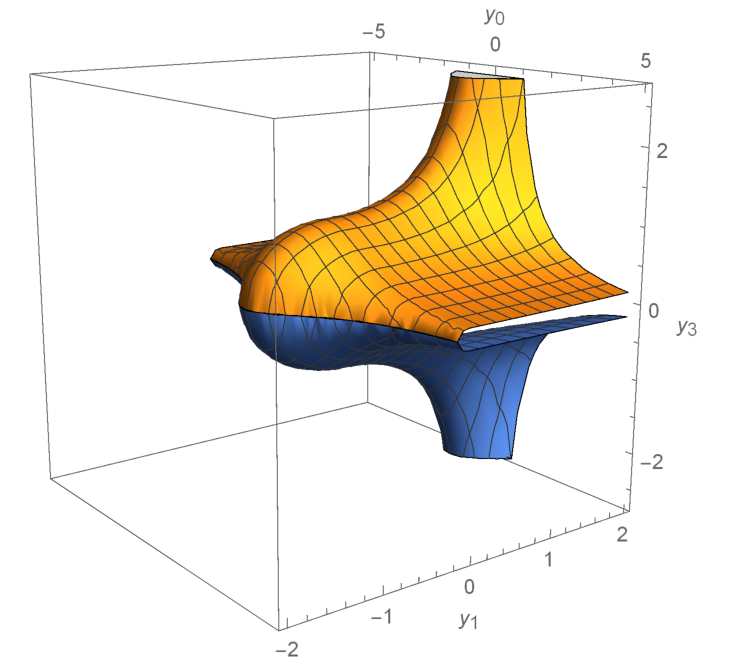
\includegraphics[width=1.1\linewidth]{Hole_with_matter_embedding.pdf}
	\caption{\label{pic_emb}The section $y^4 = y^5 = 0$ in the coordinates $ y^0 $, $ y^1 $ and $ y^3 $.}
\end{minipage}
\end{figure}

Рассмотрим явный вид вложения Фронсдала в области $r \leqslant R$ (можно найти в \cite{statja27,statja29} или \cite{frons})
\begin{align}
\label{8}	y^0_s & = 2 R \sqrt{\frac{R}{r(\tau, \chi)}-1} \cdot \ch{\left( \frac{t(\tau, \chi)}{2 R}\right)},  \\
	y^1_s & = 2 R \sqrt{\frac{R}{r(\tau, \chi)}-1} \cdot \sh{\left( \frac{t(\tau, \chi)}{2 R}\right)},  \\
\label{9}	y^2_s & = R \cdot q \left( \frac{r(\tau, \chi)}{R} \right), \\
	y^3_s &= r(\tau, \chi) \cos{\theta},  \\
	y^4_s &= r(\tau, \chi) \sin{\theta} \cos{\varphi},  \\
	y^5_s &= r(\tau, \chi) \sin{\theta} \sin{\varphi}.
\end{align}

Оказывается, что $t(\tau, \frac{\pi}{2}) \equiv 0$, поэтому $y^1$ на границе сшивки обнуляется, как и функция (\ref{0}) во вложении метрики Фридмана. Получается, что в этом случае нет необходимости расширять вложение Фронсдала до семимерного, а во вложении метрики Фридмана достаточно заменить $f(\tau)$ на две функции  (\ref{8}), (\ref{9}), взятые при $\chi = \frac{\pi}{2}$. Интересно, что в этом случае после сшивки вложение получается гладким и покрывает все значения $r>0$. Вложение оказывается шестимерным с сигнатурой $(+, -, -, -, -, -)$. Одно из его сечений представлено на Рис. \ref{pic_emb}.

\bibliographystyle{my3beznazv}
\bibliography{paston-grav-e}
\end{document} 